% chapters/06_testing.tex
\chapter{系统测试情况}

\section*{本章测试体系速览}

\begin{table}[H]
    \centering
    \begin{tabular}{p{0.15\textwidth}p{0.25\textwidth}p{0.25\textwidth}p{0.25\textwidth}}
        \toprule
        \textbf{测试层级} & \textbf{测试内容} & \textbf{用例数量} & \textbf{结果} \\
        \midrule
        单元测试 & Rust workspace 核心逻辑验证 & 13+ & 全部 PASS \\
        兼容性测试 & Linux aes-xts-plain64 逐字节比对 & 1组固定向量 & PASS \\
        正确性测试 & KVM 环境功能验证 & 12组（R01--R03、C01--C05、V01--V07） & 全部 PASS \\
        性能测试 & FIO、Filebench、SQLite、Boot & 46 PASS + 6 N/A & 全部完成 \\
        \bottomrule
    \end{tabular}
\end{table}

\begin{figure}[H]
    \centering
    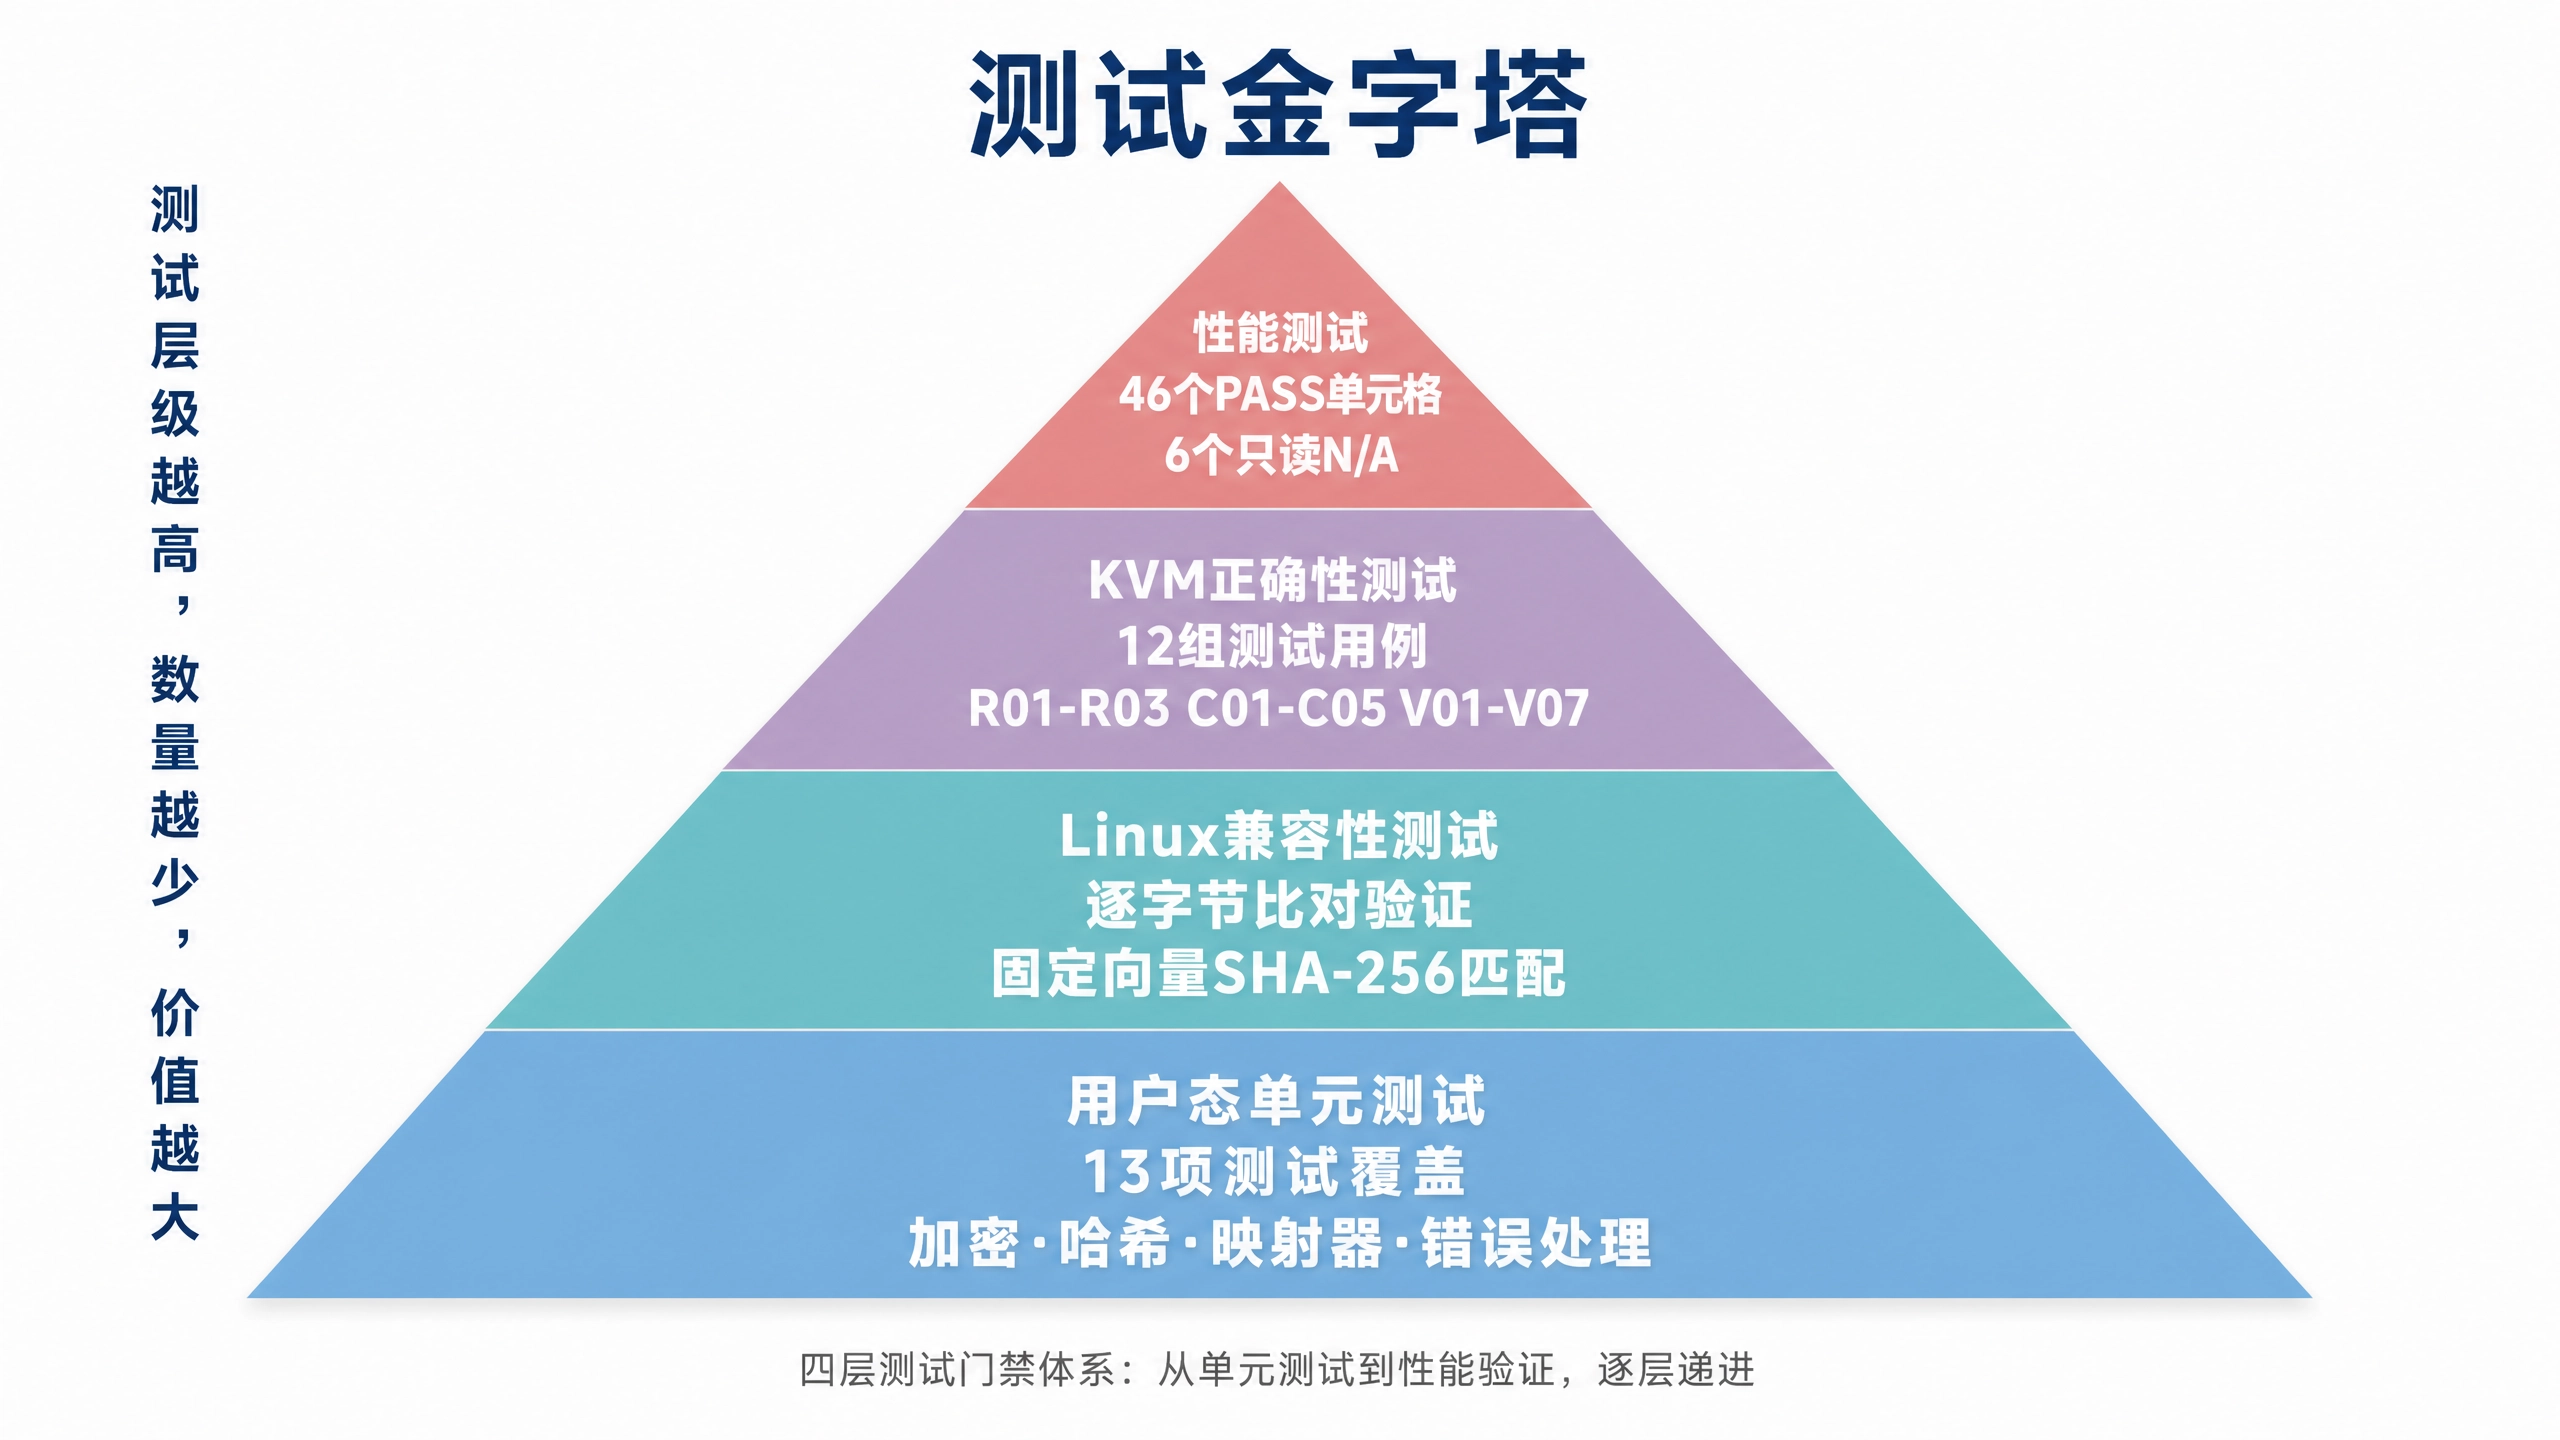
\includegraphics[width=0.85\textwidth]{test_pyramid.png}
    \caption{四层测试金字塔}
    \label{fig:test_pyramid}
\end{figure}

\section{测试体系概述}

项目采用四层门禁测试体系，自底向上逐层验证，确保功能正确性、Linux 兼容性和性能可复现性：

\begin{enumerate}
    \item \textbf{用户态单元测试（第1层）}：验证加密算法、哈希树、映射器逻辑和错误处理。在用户态快速迭代，不依赖内核环境，作为整个项目的“安全网”。入口命令：\texttt{cargo test --workspace}；
    \item \textbf{Linux 兼容性测试（第2层）}：与 Linux 内核 \texttt{aes-xts-plain64} 逐字节比对，确保密文生成与 Linux 完全一致，这是与 cryptsetup 互操作的前提。入口命令：\texttt{scripts/verify\_linux\_xts\_compat.sh}；
    \item \textbf{Asterinas KVM 正确性测试（第3层）}：在真实 VirtIO BIO 路径下验证 mapper 功能、rootfs 切换和物理损坏检测，覆盖回归、加密、完整性三大类共 12 组用例。入口命令：\texttt{tools/run\_dm\_crypt.sh}、\texttt{tools/run\_dm\_verity.sh}；
    \item \textbf{正式性能测试（第4层）}：FIO、Filebench、SQLite 和启动耗时的五轮基准，每个有效单元格固定五轮，报告中位数和标准差。入口命令：\texttt{scripts/run\_*\_matrix.sh}。
\end{enumerate}

所有测试均要求真实执行并保留原始证据（串口日志、JSON、CSV），只有满足此条件的项才标记为 \texttt{PASS}。历史无效数据（如早期假 mapper 测试）已被明确分类并隔离。

\section{测试环境基线}

\begin{table}[H]
    \centering
    \caption{正确性测试固定环境}
    \begin{tabular}{p{0.30\textwidth}p{0.60\textwidth}}
        \toprule
        \textbf{组件} & \textbf{版本/配置} \\
        \midrule
        Asterinas commit & \texttt{9d79542cadddc6164ad3f31fd8cba776969d85a9} \\
        Docker 镜像 & \texttt{asterinas/asterinas:0.18.0-20260618} \\
        镜像摘要 & \texttt{\seqsplit{sha256:7510071cb103309cc9396b970325c354713da749dfee34a807108248cc97331e}} \\
        Rust 工具链 & \texttt{nightly-2026-04-03} \\
        架构 & x86\_64 \\
        虚拟化 & QEMU/KVM，\texttt{-cpu host}，1 vCPU，8 GiB 内存 \\
        存储接口 & \texttt{virtio-blk}，符合赛题标准化要求 \\
        Cargo 缓存 & 持久化 volume（\texttt{asterinas-cargo}） \\
        rustup 缓存 & 持久化 volume（\texttt{asterinas-rustup}） \\
        \bottomrule
    \end{tabular}
\end{table}

性能测试分 Linux QEMU virtio 和 Asterinas KVM 两个平台分别执行，详细环境见 \texttt{PLATFORM\_EVAL\_ENVIRONMENT.md}。

\section{单元测试}

Rust workspace 单元测试覆盖以下核心场景（13+ 个测试用例）：

\begin{table}[H]
    \centering
    \caption{单元测试覆盖场景}
    \begin{tabular}{p{0.30\textwidth}p{0.60\textwidth}}
        \toprule
        \textbf{测试模块} & \textbf{覆盖场景} \\
        \midrule
        \texttt{crypt\_test} & dm-crypt 往返加密、错误密钥无法恢复明文 \\
        \texttt{verity\_test} & dm-verity 正常读取、篡改检测、错误根哈希拒绝、只读强制 \\
        \texttt{stack\_test} & 组合栈安全能力传播、插桩统计 \\
        \texttt{cryptsetup\_compat\_test} & Linux table 解析、offset 和 plain64 语义验证 \\
        \texttt{file\_device\_test} & 文件后端持久化、只读模式拒绝写入 \\
        \texttt{security\_boundary\_test} & 容量溢出拒绝、并发安全、不同扇区不同密文 \\
        \bottomrule
    \end{tabular}
\end{table}

\textbf{执行方式}：\texttt{cargo test --workspace}

\section{Linux 兼容性测试}

\subsection{测试目的}
确保 AES-256-XTS 实现与 Linux 内核 \texttt{aes-xts-plain64} 逐字节兼容，这是 \texttt{cryptsetup} 工具能够无缝工作的前提。

\subsection{测试方法}
\begin{enumerate}
    \item 在 Linux 系统中使用 \texttt{dmsetup} 创建 \texttt{aes-xts-plain64} 映射器；
    \item 使用相同密钥（512 位）和相同明文模式（全 0x5a 的一个扇区）分别通过 Linux 和 Rust 实现加密；
    \item 使用 \texttt{cmp} 逐字节比较两个密文；
    \item 使用 \texttt{sha256sum} 记录固定向量校验和。
\end{enumerate}

\subsection{测试结果}
\begin{itemize}
    \item 固定向量 SHA-256：\texttt{\seqsplit{4334c17f4b0380b3c1f902509cce0c0f98d9fa77aa93f6407ec940215d77921d}}
    \item 逐字节比对结果：\texttt{PASS}
    \item 证据脚本：\texttt{scripts/verify\_linux\_xts\_compat.sh}
\end{itemize}

\section{Asterinas KVM 正确性测试}

\subsection{回归测试（R01--R03）}

回归测试验证基础构建和关键用户流程的正确性，确保核心功能在每次变更后仍然正常工作。

\begin{table}[H]
    \centering
    \caption{回归测试结果}
    \begin{tabular}{p{0.12\textwidth}p{0.58\textwidth}p{0.12\textwidth}}
        \toprule
        \textbf{编号} & \textbf{测试内容与验证方法} & \textbf{结果} \\
        \midrule
        R01 & 在 Asterinas KVM 中使用真实 \texttt{cryptsetup 2.7.5} 对加密卷执行 \texttt{open}、\texttt{dd read}、\texttt{close} 完整流程，验证控制面与数据面协同工作 & \texttt{PASS} \\
        R02 & 通过 \texttt{dm\_crypt.*} 启动参数创建加密 mapper，在 initramfs 中挂载并执行 \texttt{pivot\_root} 切换到受保护根文件系统 & \texttt{PASS} \\
        R03 & 通过 \texttt{rootfs\_verity.*} 启动参数创建 verity mapper，验证 on-disk 哈希树，执行 \texttt{pivot\_root} 切换到受保护根文件系统 & \texttt{PASS} \\
        \bottomrule
    \end{tabular}
\end{table}

\textbf{证据路径}：
\begin{itemize}
    \item R01：\texttt{\seqsplit{docs/evidence/stabilization/correctness-kvm/regression/R01-cryptsetup-persistent-cache.log}}
    \item R02：\texttt{\seqsplit{docs/evidence/stabilization/correctness-kvm/regression/R02-crypt-rootfs-persistent-cache.log}}
    \item R03：\texttt{\seqsplit{docs/evidence/stabilization/correctness-kvm/regression/R03-verity-rootfs-persistent-cache.log}}
\end{itemize}

\subsection{dm-crypt 加密测试（C01--C05）}

验证 AES-256-XTS 加密的正确性，包括正确密钥、错误密钥和不同 I/O 大小的往返测试。

\begin{table}[H]
    \centering
    \caption{dm-crypt 功能测试结果}
    \begin{tabular}{p{0.12\textwidth}p{0.58\textwidth}p{0.12\textwidth}}
        \toprule
        \textbf{编号} & \textbf{测试内容与验证方法} & \textbf{结果} \\
        \midrule
        C01 & 正确密钥下通过 mapper 写入数据，读回后 SHA-256 与原始明文一致；直接读取底层设备验证为密文 & \texttt{PASS} \\
        C02 & 使用错误密钥读取 C01 写入的密文，读回数据 SHA-256 与正确明文不同，验证明文无法恢复 & \texttt{PASS} \\
        C03 & 4 KiB 块大小写入/读取往返，逐字节比对数据一致性 & \texttt{PASS} \\
        C04 & 32 KiB 块大小写入/读取往返，逐字节比对数据一致性 & \texttt{PASS} \\
        C05 & 256 KiB 块大小写入/读取往返，逐字节比对数据一致性 & \texttt{PASS} \\
        \bottomrule
    \end{tabular}
\end{table}

\textbf{证据路径}：
\begin{itemize}
    \item C01--C05：\texttt{\seqsplit{docs/evidence/stabilization/correctness-kvm/crypt/C01-C05-kvm.log}}
\end{itemize}

\subsection{dm-verity 完整性测试（V01--V07）}

验证 dm-verity 的完整性校验能力，包括正常读取和各类物理损坏场景。V03--V07 的物理篡改位置记录在 \texttt{PHYSICAL\_MUTATION\_MANIFEST.md} 中，每个用例只翻转目标块内偏移 17 的一个字节，且始终使用原始正确根哈希（不重新计算）。

\begin{table}[H]
    \centering
    \caption{dm-verity 功能测试结果}
    \begin{tabular}{p{0.12\textwidth}p{0.58\textwidth}p{0.12\textwidth}}
        \toprule
        \textbf{编号} & \textbf{测试内容与验证方法} & \textbf{结果} \\
        \midrule
        V01 & 未篡改镜像，使用正确根哈希启动，\texttt{status=verified}，根切换 PASS & \texttt{PASS} \\
        V02 & 镜像不变，仅将启动参数中的根哈希替换为错误值（修改一个字节），mapper 创建被拒绝，输出 \texttt{status=integrity-rejected} & \texttt{PASS} \\
        V03 & 物理块 0（首个数据块）偏移 17 处单字节翻转，使用原始正确根哈希，mapper 创建被拒绝 & \texttt{PASS} \\
        V04 & 物理块 32768（中间数据块）偏移 17 处单字节翻转，使用原始正确根哈希，读取返回 I/O 错误 & \texttt{PASS} \\
        V05 & 物理块 65535（最后一个数据块）偏移 17 处单字节翻转，使用原始正确根哈希，读取被拒绝 & \texttt{PASS} \\
        V06 & 物理块 65536（首个叶子哈希块）偏移 17 处单字节翻转，使用原始正确根哈希，mapper 创建被拒绝 & \texttt{PASS} \\
        V07 & 物理块 66048（首个中间哈希块）偏移 17 处单字节翻转，使用原始正确根哈希，mapper 创建被拒绝 & \texttt{PASS} \\
        \bottomrule
    \end{tabular}
\end{table}

\textbf{证据路径}：
\begin{itemize}
    \item V01：\texttt{\seqsplit{docs/evidence/stabilization/correctness-kvm/regression/R03-verity-rootfs-persistent-cache.log}}
    \item V02：\texttt{\seqsplit{docs/evidence/stabilization/correctness-kvm/corruption/V02-wrong-root.log}}
    \item V03--V07：\texttt{\seqsplit{docs/evidence/stabilization/correctness-kvm/corruption/V0[3-7]-targeted-probe.log}}
\end{itemize}

\subsection{物理篡改清单详情}

\begin{table}[H]
    \centering
    \small
    \caption{物理篡改清单（V03--V07）}
    \begin{tabular}{p{0.10\textwidth}p{0.15\textwidth}p{0.15\textwidth}p{0.20\textwidth}p{0.30\textwidth}}
        \toprule
        \textbf{编号} & \textbf{篡改区域} & \textbf{物理块号} & \textbf{字节偏移} & \textbf{篡改后块 SHA-256} \\
        \midrule
        V03 & 首个数据块 & 0 & 17 & \texttt{b31dc2a37cc0c3c1...} \\
        V04 & 中间数据块 & 32768 & 134217745 & \texttt{1e12a90f8a205a6a...} \\
        V05 & 最后一个数据块 & 65535 & 268431377 & \texttt{dbeaf0b712cd66aa...} \\
        V06 & 首个叶子哈希块 & 65536 & 268435473 & \texttt{5026ae43d7fd0385...} \\
        V07 & 首个中间哈希块 & 66048 & 270532625 & \texttt{557feb6640edc47d...} \\
        \bottomrule
    \end{tabular}
\end{table}

所有篡改均只翻转一个字节，且\textbf{继续使用原始正确根哈希}（\texttt{b1a6dcd4...}），验证了 dm-verity 的篡改检测能力不依赖于重新计算根哈希。

\section{性能测试}

性能测试遵循 \texttt{docs/benchmark\_contract.md} 中定义的合同，所有有效单元格固定运行五轮，报告均值、中位数和标准差，不剔除异常值。Linux 与 Asterinas 结果分平台列示，不进行跨平台倍率比较。

\subsection{FIO 矩阵}

FIO 矩阵覆盖 4 KiB、32 KiB、256 KiB 三种块大小，顺序/随机读/写四种操作，QD=1（额外 4 KiB randread QD=16）。

\begin{table}[H]
    \centering
    \caption{FIO 矩阵完成情况}
    \begin{tabular}{p{0.35\textwidth}p{0.22\textwidth}p{0.22\textwidth}}
        \toprule
        \textbf{范围} & \textbf{有效单元格} & \textbf{结果} \\
        \midrule
        Asterinas KVM dm-crypt & 13 项 $\times$ 5 轮 & \texttt{PASS} \\
        Asterinas KVM dm-verity & 7 项 $\times$ 5 轮 & \texttt{PASS}（6 项 N/A） \\
        Linux QEMU virtio raw & 13 项 $\times$ 5 轮 & \texttt{PASS} \\
        Linux QEMU virtio dm-crypt & 13 项 $\times$ 5 轮 & \texttt{PASS} \\
        Linux QEMU virtio dm-verity 读 & 7 项 $\times$ 5 轮 & \texttt{PASS}（6 项 N/A） \\
        \bottomrule
    \end{tabular}
\end{table}

\textbf{代表性结果（五轮中位带宽，MiB/s）}：

Asterinas 256 MiB 正式合同（4 KiB 同步读、QD1；相对值为配对 raw，不与下表 8.908 / 7.505 混算）：

\begin{table}[H]
    \centering
    \begin{tabular}{p{0.28\textwidth}p{0.22\textwidth}p{0.22\textwidth}}
        \toprule
        \textbf{设备} & \textbf{中位吞吐} & \textbf{相对配对 raw} \\
        \midrule
        raw（两组共十轮） & 4.249 & 100.0\% \\
        dm-crypt & 4.059 & 95.6\% \\
        dm-verity & 3.815 & 87.3\% \\
        \bottomrule
    \end{tabular}
\end{table}

同一宿主机、KVM、CPU=\texttt{host}、1 vCPU、8\,GiB、同一 virtio-blk 数据盘前 256\,MiB、4\,KiB、\texttt{sync}、\texttt{direct=1}、QD1 的 Linux guest 对照如下。dm-crypt 保留率相对表中 raw 列；dm-verity 保留率相对配对 raw（Linux 4.641、Asterinas 4.368）。Asterinas 相对 Linux guest 的绝对吞吐为 raw 82.4\%、dm-crypt 85.5\%、dm-verity 87.3\%（$3.815/4.369$）。自身保留率不代表绝对吞吐超过 Linux。

\begin{table}[H]
    \centering
    \small
    \caption{Linux guest 与 Asterinas 同条件对照（MiB/s）}
    \begin{tabular}{lrrrrr}
        \toprule
        \textbf{系统} & \textbf{raw} & \textbf{dm-crypt} & \textbf{crypt 保留率} & \textbf{dm-verity} & \textbf{verity 保留率} \\
        \midrule
        Linux guest & 5.150 & 4.746 & 92.158\% & 4.369 & 94.1\% \\
        Asterinas & 4.245 & 4.059 & 95.621\% & 3.815 & 87.3\% \\
        \bottomrule
    \end{tabular}
\end{table}

\begin{figure}[H]
    \centering
    \includegraphics[width=0.92\textwidth]{linux_asterinas_4k_sync_throughput.png}
    \caption{4\,KiB sync QD1 中位吞吐：Linux guest 与 Asterinas}
    \label{fig:linux_asterinas_4k_sync_throughput}
\end{figure}

\begin{figure}[H]
    \centering
    \includegraphics[width=0.92\textwidth]{linux_asterinas_4k_sync_retention.png}
    \caption{Mapper 保留率：crypt 相对表中 raw，verity 相对配对 raw}
    \label{fig:linux_asterinas_4k_sync_retention}
\end{figure}

\begin{table}[H]
    \centering
    \begin{tabular}{p{0.25\textwidth}p{0.15\textwidth}p{0.15\textwidth}p{0.18\textwidth}p{0.18\textwidth}}
        \toprule
        \textbf{负载} & \textbf{块大小} & \textbf{QD} & \textbf{Linux raw} & \textbf{Linux dm-crypt} \\
        \midrule
        read & 4 KiB & 1 & 11.391 & 10.942 \\
        read & 256 KiB & 1 & 134.623 & 129.474 \\
        randread & 4 KiB & 16 & 58.931 & 58.947 \\
        randwrite & 256 KiB & 1 & 130.124 & 109.453 \\
        \bottomrule
    \end{tabular}
\end{table}

\begin{table}[H]
    \centering
    \begin{tabular}{p{0.25\textwidth}p{0.15\textwidth}p{0.15\textwidth}p{0.18\textwidth}p{0.18\textwidth}}
        \toprule
        \textbf{负载} & \textbf{块大小} & \textbf{QD} & \textbf{Asterinas dm-crypt} & \textbf{Asterinas dm-verity} \\
        \midrule
        read & 4 KiB & 1 & 8.908 & 7.505 \\
        read & 256 KiB & 1 & 97.456 & 53.363 \\
        randread & 4 KiB & 16 & 8.614 & 4.618 \\
        randwrite & 256 KiB & 1 & 93.541 & N/A（只读） \\
        \bottomrule
    \end{tabular}
\end{table}

\textbf{证据路径}：Linux QEMU virtio FIO 见 \texttt{docs/evidence/linux-qemu-fio-20260816/}；Asterinas FIO 见 \texttt{docs/evidence/final-performance-20260811/PERFORMANCE\_MATRIX.csv}。

\subsection{补充性能测试}

\begin{table}[H]
    \centering
    \caption{补充性能测试结果（五轮中位数）。Filebench 与 SQLite 为 Linux QEMU/KVM guest；启动耗时为 Asterinas。}
    \begin{tabular}{p{0.35\textwidth}p{0.18\textwidth}p{0.18\textwidth}p{0.18\textwidth}}
        \toprule
        \textbf{测试} & \textbf{raw/plain} & \textbf{dm-crypt} & \textbf{dm-verity} \\
        \midrule
        Filebench fileserver（ops/s） & 27855.155 & 25666.016 & N/A \\
        Filebench fileserver（MB/s） & 656.9 & 605.0 & N/A \\
        SQLite 10000 行总耗时（s） & 0.138095 & 0.143336 & 0.001151（只读查询） \\
        Asterinas 启动耗时（s） & 51.331303 & 51.629820 & 52.743415 \\
        \bottomrule
    \end{tabular}
\end{table}

SQLite dm-verity 只执行查询阶段，不能与完整写事务总耗时横比。启动耗时从 QEMU 进程启动计至串口出现受保护根文件系统 PASS 标记。

\textbf{证据路径}：
\begin{itemize}
    \item Filebench / SQLite（Linux QEMU guest）：\texttt{\seqsplit{docs/evidence/linux-qemu-filebench-sqlite-20260817/}}
    \item Boot：\texttt{docs/evidence/final-performance-20260811/boot-matrix/}
\end{itemize}

\section{复现命令}

以下命令提供了从单元测试到性能验证的完整复现路径，确保所有测试结果均可独立验证：

\begin{verbatim}
# 第1层：用户态单元测试
cargo test --workspace

# 第2层：Linux 兼容性测试
sudo bash scripts/verify_linux_xts_compat.sh

# 第3层：Asterinas KVM 正确性测试
# R01--R03、C01--C05、V01--V07 的完整环境变量与命令见仓库根目录 README

# 第4层：正式性能测试（分平台执行，每个工况五轮）
sudo bash scripts/run_fio_matrix.sh --platform linux-host --runs 5
bash scripts/run_fio_matrix.sh --platform asterinas-kvm \
  --asterinas-dir "$PWD/asterinas" --runs 5

# 补充性能测试
sudo RUNS=5 bash scripts/run_filebench_matrix.sh
sudo RUNS=5 ROWS=10000 bash scripts/run_sqlite_matrix.sh
RUNS=5 ENABLE_KVM=1 bash scripts/run_boot_matrix.sh

# 静态检查与证据验证
python3 scripts/check_benchmark_package.py
python3 scripts/verify_kvm_evidence.py
python3 scripts/review_release_check.py
\end{verbatim}

所有测试命令的详细说明和参数配置见仓库根目录 \texttt{README.md} 和 \texttt{\seqsplit{docs/benchmark\_contract.md}}。
\section{数据真实性与审计}

\subsection{历史问题处理}
早期 Asterinas dm-crypt FIO 测试中，mapper 设备未正确创建（因启动参数错误或自检失败），但测试脚本继续执行，fio 将不存在的设备路径（如 \texttt{\seqsplit{/dev/mapper/dm-crypt-bench}}）当作普通文件创建并测试，产生了数量级异常的数据（高达数千 MiB/s）。

该批次结果被明确分类为 \texttt{HARNESS\_BUG}，已从正式矩阵中移除。重新执行的测试使用修复后的 runner（增加设备存在性检查），确保每个数据点均来自 guest 内真实 mapper 设备。

\subsection{正式数据标准}
\begin{itemize}
    \item 每个有效单元格包含 5 轮原始 JSON/CSV；
    \item 每轮测试均保留完整的 fio 输出和环境 metadata；
    \item 报告中位数和标准差，不选择最好一轮；
    \item 旧数据、失败重试和调试日志不进入最终目录；
    \item 生成器脚本不读取无效数据目录。
\end{itemize}

\section{静态检查与门禁}

项目包含自动化静态检查脚本，确保提交材料的完整性和一致性：

\begin{lstlisting}[basicstyle=\ttfamily\small, breaklines=true]
python3 scripts/check_benchmark_package.py
python3 scripts/verify_kvm_evidence.py
python3 scripts/review_release_check.py
\end{lstlisting}

检查内容包括：
\begin{itemize}
    \item 必要证据文件是否存在（kernel build 日志、R01--R03、C01--C05、V02--V07）；
    \item 最终 FIO 矩阵是否包含 46 个 PASS 单元格；
    \item 每个 PASS 单元格是否关联 5 轮原始数据；
    \item 启动矩阵是否包含 plain、dm-crypt、dm-verity 各至少 5 轮；
    \item 公开文档中是否存在无证据支持的性能夸大表述。
\end{itemize}

\section{证据可复核性}

所有正式测试证据均以原始形式保存，便于复核：

\begin{table}[H]
    \centering
    \caption{证据目录结构}
    \begin{tabular}{p{0.35\textwidth}p{0.55\textwidth}}
        \toprule
        \textbf{路径} & \textbf{内容} \\
        \midrule
        \texttt{\seqsplit{stabilization/build-recovery/}} & kernel build 日志 \\
        \texttt{\seqsplit{stabilization/correctness-kvm/regression/}} & R01--R03 串口日志 \\
        \texttt{\seqsplit{stabilization/correctness-kvm/crypt/}} & C01--C05 串口日志 \\
        \texttt{\seqsplit{stabilization/correctness-kvm/corruption/}} & V02--V07 串口日志 \\
        \texttt{\seqsplit{final-performance-20260811/}} & 最终性能矩阵、报告、原始数据 \\
        \texttt{\seqsplit{final-performance-20260811/asterinas-fio/}} & Asterinas KVM FIO 原始 JSON \\
        \texttt{\seqsplit{linux-qemu-fio-20260816/}} & Linux QEMU virtio FIO 原始 JSON \\
        \texttt{\seqsplit{linux-qemu-filebench-sqlite-20260817/}} & Linux QEMU guest Filebench / SQLite \\
        \texttt{\seqsplit{final-performance-20260811/filebench-valid/}} & Linux host Filebench 归档，不再引用 \\
        \texttt{\seqsplit{final-performance-20260811/sqlite/}} & Linux host SQLite 归档，不再引用 \\
        \texttt{\seqsplit{final-performance-20260811/boot-matrix/}} & 启动 15 轮记录 \\
        \texttt{stack/} & 组合栈启动证据 \\
        \bottomrule
    \end{tabular}
\end{table}

每条矩阵记录都包含原始证据相对路径，不依赖手工修改数字。完整的复现命令和证据索引见仓库根目录 \texttt{README.md} 和 \texttt{docs/evidence/README.md}。

\section{测试门禁汇总}

\begin{table}[H]
    \centering
    \caption{全部测试门禁状态}
    \begin{tabular}{p{0.30\textwidth}p{0.20\textwidth}p{0.40\textwidth}}
        \toprule
        \textbf{测试门禁} & \textbf{结果} & \textbf{证据位置} \\
        \midrule
        Rust workspace 单元测试 & \texttt{PASS} & \texttt{cargo test} \\
        Linux XTS 逐字节兼容 & \texttt{PASS} & \texttt{verify\_linux\_xts\_compat.sh} \\
        R01--R03 回归测试 & \texttt{PASS} & \texttt{correctness-kvm/regression/} \\
        C01--C05 加密功能 & \texttt{PASS} & \texttt{correctness-kvm/crypt/} \\
        V01--V07 完整性校验 & \texttt{PASS} & \texttt{correctness-kvm/corruption/} \\
        FIO 性能矩阵（46 PASS） & \texttt{PASS} & \texttt{final-performance-20260811/} \\
        Filebench（5+5 轮） & \texttt{PASS} & \texttt{\seqsplit{linux-qemu-filebench-sqlite-20260817/filebench/}} \\
        SQLite（5+5+5 轮） & \texttt{PASS} & \texttt{\seqsplit{linux-qemu-filebench-sqlite-20260817/sqlite/}} \\
        Boot 耗时（5+5+5 轮） & \texttt{PASS} & \texttt{\seqsplit{final-performance-20260811/boot-matrix/}} \\
        静态包检查 & \texttt{PASS} & \texttt{review\_release\_check.py} \\
        \bottomrule
    \end{tabular}
\end{table}

\section{小结}

所有 P0 正确性测试（R01--R03、C01--C05、V01--V07）全部通过，正式性能矩阵包含 46 个有效单元格和 6 个只读 N/A，补充测试（Filebench、SQLite、Boot）均完成五轮验证。

历史无效数据（如早期假 mapper 测试、失败重试）已被明确分类为 \texttt{HARNESS\_BUG} 并隔离，不进入最终结论。尚未定义 runner 的扩展 P1 项保持 \texttt{UNTESTED}，不解释为 PASS，也不解释为产品失败。

完整测试证据已全部归档至 \texttt{docs/evidence/} 目录，所有原始日志、JSON、CSV 均可复核。本章列出的全部复现命令（\texttt{cargo test}、\texttt{verify\_linux\_xts\_compat.sh}、\texttt{run\_fio\_matrix.sh}、\texttt{run\_filebench\_matrix.sh}、\texttt{run\_sqlite\_matrix.sh}、\texttt{run\_boot\_matrix.sh}、\texttt{check\_benchmark\_package.py}、\texttt{verify\_kvm\_evidence.py}、\texttt{review\_release\_check.py}）为所有测试结果提供了完整的可复现入口。测试结果全面覆盖赛题五项技术指标，为项目的正确性和性能提供了可验证的支撑。